%%%%%%%%%%%%%%%%%%%%%%%%%%%%%%%%%%%%%%%%%%%%%%%%%%%%%%%%%%%%%%%%%%%%%%%%%%%%%%%%%
%																				%
%	TRABAJO:	Trabajo Final													%
%				Especialidad en Ingenier�a en Sistemas de Informaci�n			%
%																				%
%		Titulo:																	%
%																				%
%		Autor:	Juli�n Nonino													%
%																				%
%	Capitulo sobre Dise�o de la Arquitectura									%	
%																				%
%	A�o: 2016																	%
%																				%
%%%%%%%%%%%%%%%%%%%%%%%%%%%%%%%%%%%%%%%%%%%%%%%%%%%%%%%%%%%%%%%%%%%%%%%%%%%%%%%%%

\chapter{Dise�o de la Arquitectura del Sistema}
\label{chapter_arquitectura}


\begin{figure}[H]
	\centering
	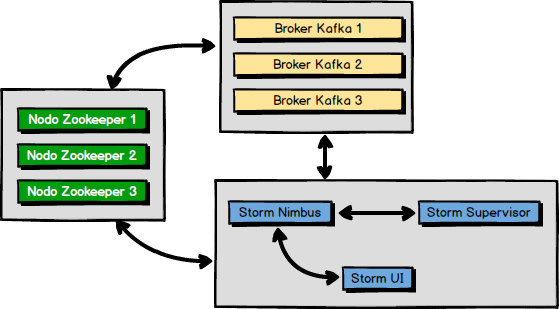
\includegraphics[width=1\linewidth]{./informe/desarrollo/img/ArquitecturaServidor}
	\caption{Arquitectura general del Cl�ster incluyendo Zookeeper, Kafka y Storm}
\end{figure}

\begin{figure}[H]
	\centering
	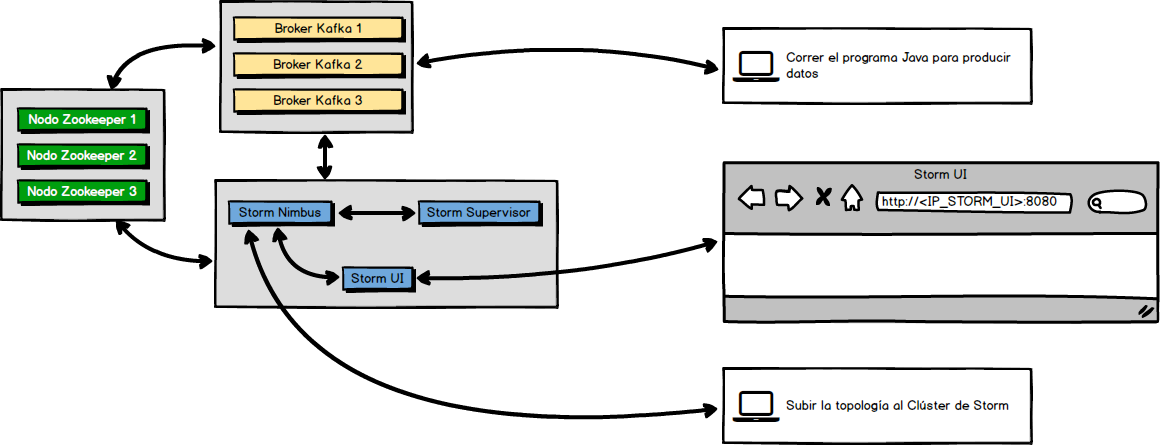
\includegraphics[width=1\linewidth]{./informe/desarrollo/img/ArquitecturaConexionClientes}
	\caption{Arquitectura general del Cl�ster conectado a los programas cliente}
\end{figure}